%%%%%%%%%%%%%%%%%%%%%%%%%%%%%%%%%%%%%%%%%%%%%%%%%%%%%%%%%%%%%%%%%%%%%%%%%%%%
%% Author style for INFORMS Transactions on Education (ited)
%% Mirko Janc, Ph.D., INFORMS, pubtech@informs.org
%% ver. 0.92, June 2009 -- default options: single-spaced, double-blinded
%%%%%%%%%%%%%%%%%%%%%%%%%%%%%%%%%%%%%%%%%%%%%%%%%%%%%%%%%%%%%%%%%%%%%%%%%%%%
%\documentclass[ited]{informs3}                      % for a regular run
%\documentclass[ited,nonblindrev]{informs3}          % for review, not blinded
%\documentclass[ited,blindrev,copyedit]{informs3}    % spaced for copyediting
\documentclass[ited,blindrev]{informs3}              % for review, blinded

\usepackage[most]{tcolorbox}
\usepackage{minted}
\tcbuselibrary{minted} % tcolorbox minted library, required to use the "minted" tcb listing engine (this library is not loaded by the option [most])
\usepackage[colorlinks]{hyperref} % ALWAYS load this package LAST



% If hyperref is used, dvi-to-ps driver of choice must be declared as
%   an additional option to the \documentstyle. For example
%\documentclass[dvips,ited]{informs1}      % if dvips is used 
%\documentclass[dvipsone,ited]{informs1}   % if dvipsone is used, etc. 

% Private macros here (check that there is no clash with the style)
\newcommand{\code}[1]{\texttt{#1}}

% Natbib setup for author-year style
\usepackage{natbib}
 \bibpunct[, ]{(}{)}{,}{a}{}{,}%
 \def\bibfont{\small}%
 \def\bibsep{\smallskipamount}%
 \def\bibhang{24pt}%
 \def\newblock{\ }%
 \def\BIBand{and}%

%% Setup of theorem styles. Outcomment only one. 
%% Preferred default is the first option.
\TheoremsNumberedThrough     % Preferred (Theorem 1, Lemma 1, Theorem 2)
%\TheoremsNumberedByChapter  % (Theorem 1.1, Lema 1.1, Theorem 1.2)

%% Setup of the equation numbering system. Outcomment only one.
%% Preferred default is the first option.
\EquationsNumberedThrough    % Default: (1), (2), ...
%\EquationsNumberedBySection % (1.1), (1.2), ...

% In the reviewing and copyediting stage enter the manuscript number.
%\MANUSCRIPTNO{} % When the article is logged in and DOI assigned to it,
                 %   this manuscript number is no longer necessary

%%%%%%%%%%%%%%%%
\begin{document}
%%%%%%%%%%%%%%%%

% Outcomment only when entries are known. Otherwise leave as is and 
%   default values will be used.
%\setcounter{page}{1}
%\VOLUME{00}%
%\NO{0}%
%\MONTH{Xxxxx}% (month or a similar seasonal id)
%\YEAR{0000}% e.g., 2005
%\FIRSTPAGE{000}%
%\LASTPAGE{000}%
%\SHORTYEAR{00}% shortened year (two-digit)
%\ISSUE{0000} %
%\LONGFIRSTPAGE{0001} %
%\DOI{10.1287/xxxx.0000.0000}%

% Author's names for the running heads
% Sample depending on the number of authors;
% \RUNAUTHOR{Jones}
% \RUNAUTHOR{Jones and Wilson}
% \RUNAUTHOR{Jones, Miller, and Wilson}
% \RUNAUTHOR{Jones et al.} % for four or more authors
% Enter authors following the given pattern:
\RUNAUTHOR{Isken}

% Title or shortened title suitable for running heads. Sample:
% \RUNTITLE{Bundling Information Goods of Decreasing Value}
% Enter the (shortened) title:
\RUNTITLE{Spreadsheet modeling with Python}

% Full title. Sample:
% \TITLE{Bundling Information Goods of Decreasing Value}
% Enter the full title:
\TITLE{Spreadsheet modeling with Python}

% Block of authors and their affiliations starts here:
% NOTE: Authors with same affiliation, if the order of authors allows, 
%   should be entered in ONE field, separated by a comma. 
%   \EMAIL field can be repeated if more than one author
\ARTICLEAUTHORS{%
\AUTHOR{Mark W. Isken}
\AFF{Oakland University, \EMAIL{isken@oakland.edu}, \URL{http://www.sba.oakland.edu/faculty/isken/}}
% Enter all authors
} % end of the block

\ABSTRACT{%
TODO: Text of your abstract % Enter your abstract
}%

% Sample
%\KEYWORDS{deterministic inventory theory; infinite linear programming duality; 
%  existence of optimal policies; semi-Markov decision process; cyclic schedule}

% Fill in data. If unknown, outcomment the field
\KEYWORDS{python, spreadsheet modeling}
\HISTORY{}

\maketitle
%%%%%%%%%%%%%%%%%%%%%%%%%%%%%%%%%%%%%%%%%%%%%%%%%%%%%%%%%%%%%%%%%%%%%%

% Samples of sectioning (and labeling) in ITED
% NOTE: (1) \section and \subsection do NOT end with a period
%       (2) \subsubsection and lower need end punctuation
%       (3) capitalization is as shown (title style).
%
%\section{Introduction.}\label{intro} %%1.
%\subsection{Duality and the Classical EOQ Problem.}\label{class-EOQ} %% 1.1.
%\subsection{Outline.}\label{outline1} %% 1.2.
%\subsubsection{Cyclic Schedules for the General Deterministic SMDP.}
%  \label{cyclic-schedules} %% 1.2.1
%\section{Problem Description.}\label{problemdescription} %% 2.

% Text of your paper here

\section{Introduction}

Spreadsheet based modeling has transformed the teaching of management science in business schools over the past three decades. The late 1990's saw first editions of game changing textbooks \cite{winstonPracticalManagementScience2018,ragsdaleSpreadsheetModelingDecision2017} focused on the use of spreadsheets in teaching modeling and management science.  A series of conferences focused on teaching management science (TMS) with spreadsheets started at Dartmouth in 1998 and several presentations from that conference made up the bulk of papers in the first two issues of the INFORMS Transactions on Education journal. The next few decades saw numerous textbooks \cite{BusinessAnalyticsArt, BusinessAnalytics4th} and teaching papers \cite{INFORMSTransactionsEducation2014} that prominently featured spreadsheet based modeling.

Despite numerous calls for and predictions of the eradication of spreadsheets from the business world, Excel and other spreadsheets are alive and well. Yes, spreadsheets have well known limitations. Spreadsheets are not databases and probably should not be used as one, especially for relational data models. There are better data visualization and exploration tools. There are better dashboarding tools that are more easily maintained in a production environment. Spreadsheet errors can be a huge problem. Version control and documentation present challenges. There are data size limitations and external data links present their own set of challenges. But, Excel continues to be used for a wide range of quantitative analysis related activities throughout the business world. One particular use is the building and exercising of models of business problems
to explore the impact of various model inputs on key outputs. This ``what if?'' type modeling is facilitated by Excel's flexibility, numerous built in functions, integrated sensitivity analysis via \href{https://support.microsoft.com/en-us/office/calculate-multiple-results-by-using-a-data-table-e95e2487-6ca6-4413-ad12-77542a5ea50b}{Data Tables},  \href{https://support.microsoft.com/en-us/office/use-goal-seek-to-find-the-result-you-want-by-adjusting-an-input-value-320cb99e-f4a4-417f-b1c3-4f369d6e66c7}{Goal
	Seek} or break-even analysis and visualization capabilities. 

At the same time, the analytics world has been changing. The advent of programmatic analytics using tools like R and Python have changed the practice of analytics as well as the teaching landscape. Limitations of spreadsheets with respect to reproducibility and automation have certainly played a role.  Additionally, both R and Python are free, open source, and have a rich set of analytics related libraries that have contributed to their growing popularity. Python, being a general purpose programming language, also offers advantages when moving models and analytical analysis pipelines from the prototype stage into production. Enormous data science ecosystems have emerged around both R and Python providing a wealth of learning resources for both new and experienced analytics students and professionals.

Numerous R and Python based data science courses have been developed and offered at universities and through online learning platforms such as Coursera, EdX, Udemy and others. Some of these courses have made a large amount of their course content freely available for self-learners and for other educators.  In 2015, we created a course called \href{http://www.sba.oakland.edu/faculty/isken/courses/mis5470/}{Practical Computing for Data Analytics} (PCDA) that introduced both R and Python (along with a little Linux) for use in data analytics work. This new course was meant as a follow up to the \href{http://www.sba.oakland.edu/faculty/isken/courses/mis5460/}{spreadsheet based modeling course} we have had in place since 2001.

The PCDA course, like many introductory data science courses, focuses mostly on data wrangling, exploratory data analysis (EDA), and statistical/machine learning based predictive models. In teaching EDA using tools like ggplot2, students are challenged to think about how they would go about trying to use Excel to create some of the plots that are easy to do with R and Python based plotting libraries. There is some limited coverage of using Python to open Excel files and do worksheet manipulation. However, other than a Python based simulation of the Monte Hall 3-door problem, there was no real attempt to do the kind of modeling that is the focus of most spreadsheet based modeling textbooks. 

Python has continued to make inroads to analytical territory that was formerly dominated by spreadsheets. The widely used Python data analysis library, pandas, was created by Wes McKinney while working as a quantitative financial analyst \cite{PythonDataAnalysis}. Python is widely used for data wrangling, visualization and predictive modeling using various flavors of regression, tree based models and neural networks. You can get a very good sense of this by visiting the very popular \href{https://www.reddit.com/r/datascience/}{r/datascience subreddit on Reddit} -- a well known online forum. But, it got me to thinking. What about those things for which Excel is particularly well suited such as building formula based models and doing sensitivity analysis on these models? What would those look like in Python? The importance of modeling, articulated so well in the pages of this journal \cite{powellTeachingModelingManagement2001}, has not abated. What role does Python have to play in supporting the kind of modeling taught for years in our business schools?

In 2021, I published a \href{https://bitsofanalytics.org/#category=excel}{series of blog posts} that explored this question and formed the basis of the teaching module described in this paper. During the development of these posts, I came across the \href{https://quantecon.org/}{Quant Econ: open source code for economic modeling} project which \quote{is a nonprofit organization dedicated to development and documentation of open source computational tools for economics, econometrics, and decision making}. This is a mature project, run by renowned economists, with significant support. They have developed and released numerous high quality Jupyter notebooks exploring a range of computational economic and financial modeling topics. Here was an example of the Python for business usage I had been seeking. With this as inspiration, I decided to turn my blog post series into a teaching module called Excel with Python (EwP). 

The EwP module is not as polished nor as advanced as the Quant Econ materials, but does add to the growing body of freely available teaching materials aimed at Python for business modeling. My goals for EwP are also a little different than those of Quant Econ and include:

\begin{itemize}
	\item teaching relevant and more advanced Python to business students using familiar and simple modeling examples,
	\item conveying a sense of the software design and development process,
	\item acting as a tour guide for a learning journey,
	\item teaching students to think and act like a software developer, not just an analyst.
\end{itemize}

Recently there has been more recognition of the need for data scientists to learn basic software engineering principes \cite{SoftwareEngineeringData,SoftwareEngineeringDataa,BuildingReproducibleAnalytical}.  The image of newly minted data science graduates developing spaghetti coded Jupyter notebooks not nearly ready for being put into production has reached \href{https://www.reddit.com/r/ProgrammerHumor/comments/y2xe3n/like_every_time_ever_when_the_devops_engineer/}{meme like status}. I hoped to address some of these issues in the EwP module. Sneakily, students would be exposed to some simple software engineering concepts during the process of building and analyzing familiar models. This is really no different than the integration of advanced Excel functions and techniques with spreadsheet modeling tutorials. Just as spreadsheet modeling students were able to easily wow their coworkers and managers with INDEX-MATCH and intermediate Pivot Table skills, I hoped that my students ability to properly document a Python function and use git and GitHub would give them a bit more professional credibility.

We will begin with a brief discussion of the overall positioning and structure of the EwP module within our business analytics programs. Then, each of the three main EwP submodules are described in some detail. Finally we conclude with a brief discussion of our experience in delivering this module and plans for the future.

\section{Module positioning and structure}

At our institution, The EwP module is part of a business course entitled ``Advanced Analytics with Python'' (\href{http://www.sba.oakland.edu/faculty/isken/courses/mis6900}{AAP}). The students taking this course have already taken the PCDA course within which they learned fundamental Python programming within the context of data analytics over seven weeks. The PCDA course ends with intro to the \href{https://scikit-learn.org/stable/index.html}{scikit-learn library} for doing predictive modeling in Python and the AAP course begins where the PCDA course ends. The EwP module could also be used as part of a semester long Python based analytics course. Most AAP students have also already taken "Business Analytics" (\href{http://www.sba.oakland.edu/faculty/isken/courses/mis5460}{BA}) which is a spreadsheet based introduction to business analytics. We do not strictly require the spreadsheet based course be taken before the PCDA or AAP courses as that course draws students from outside of our business programs who are strictly interested in programmatic tools such as Python. The BA and PCDA courses have historically been offered in face to face mode in a computer teaching lab. Since 2020, these two courses have been also offered as online, asynchronous courses. The newer AAP course has been offered since 2021 in an online asynchronous mode. All three courses have \href{http://www.sba.oakland.edu/Faculty/isken/teaching.html}{extensive course websites} that are publicly accessible, including access to all of the video content and supporting files. 

What kind of Python background do students need to have in order to be ready for the EwP module? A basic familiarity with Python fundamentals for data analysis is required, including:

\begin{itemize}
	\item variables, arithmetic and boolean operators, and basic data types,
	\item data structures such as lists, dictionaries, tuples, NumPy arrays and pandas dataframes,
	\item flow control such as branching with \texttt{if \ldots else} and looping with \texttt{for} and \texttt{while}
	\item module imports,
	\item using built in functions and accessing methods and properties of objects,
	\item creating functions,
	\item basic use of NumPy and pandas for data wrangling and analysis,
	\item basic plotting with matplotlib.
\end{itemize}

The EwP module is made up of three submodules. The first of these focuses on building and using a typical spreadsheet model using Python. Then the functionality developed in the first submodule is deployed as a reusable package. The final submodule is an introduction to using Python to manipulate Excel files.

All of the Python modules in the PCDA course as well as the entire AAP course are taught using a combination of Jupyter notebooks, Python scripts, and videos walking through the notebooks. Jupyter notebooks, part of \href{https://jupyter.org/}{Project Jupyter}, are an example of \textit{literate computing} \cite{Jupyter_proposal} and allow one to create educational narratives that support iterative exploration and development. The ability to weave standard explanatory language with formal programming languages has made notebook computing a defacto standard in the data science education community \cite{perkel2018jupyter}. Jupyter notebooks can also include equations written in \LaTeX, data visualizations, and other multi-media. The technology is free, open source, runs on most computing platforms, and has a huge user community that has created a large number of resources for students, faculty and industry practitioners. 

Central to Jupyter notebooks is a mix of \textit{code cells} and \textit{markdown cells}. Code cells contain executable code while markdown cells contain plain text using \href{URL}{markdown} for styling text. For example, Figure \ref{cells_edit_model} shows two markdown cells separated by a code cell as they look when in editing mode. After running the cells, they appear as show in Figure \ref{cells_after_running}. Mixing code and markdown cells makes it quite easy to create interactive tutorials in which students can not only run pre-written code, but can also add their own code -- all with the aid of supporting explanatory text. All of the blog posts upon which EwP is based were written in Jupyter notebooks. There are countless introductory tutorials for Jupyter notebooks, but the official Project Jupyter Documentations \cite{ProjectJupyterDocumentation} is a very good place to start if you are new to notebook computing.


\section{Submodule 1: What-if analysis with Python}

There are two overarching learning objectives for this first set of Jupyter notebooks. Students learn how Python might be used to do something they are quite familiar with doing in a spreadsheet -- model building and sensitivity analysis. At the same time, students encounter, as needed, more advanced Python programming concepts and techniques. In this way, the computational problem to be solved drives the introduction of more advanced Python concepts and techniques instead of such things being presented in a vacuum. I make it a point to show that there are often multiple possible approaches to a computational problem by being willing to abandon one approach and trying another. Emphasis is given to the lessons learned from each path explored. Every notebook is accompanied by screencasts that walk the students through the material and act as a guided tour with challenges to overcome along the way. The screenshot in \ref{fig:activities} shows the portion of the course web page that provides the high level roadmap through the notebooks and associated screencasts.
 
 
\subsection{Notebook 1: Modeling and data tables}

The stage is set with an overview of a typical spreadsheet based model that most of the students have seen before. See Figure \ref{fig:xl_model} for a screenshot of the Excel model.

\begin{tcolorbox}
\begin{quotation}
\textsf{	
	It's a really simple model in which we are selling a single product that we produce. There is a fixed cost to producing the product as well as a variable production cost per unit. We can sell the product for some price and we believe that demand for the product is related to the selling price through a power function. Let's assume for now that we have sufficient capacity to produce to demand and that all inputs are deterministic (we'll deal with simulating uncertainty later in this document).}
	
	\textsf{The details aren't so important right now as is the overall structure of the model. There are a few key inputs and some pretty straightforward formulas for computing cost, revenue and profit. Notice the 1-way Data Table being used to explore how profit varies for different selling prices. There's a graph driven by the Data Table and some Text Boxes used for annotation and summary interpretative comments. There's a button that launches Goal Seek to find the break even selling price and a 2-way Data Table (not shown) to explore the joint effect of selling price and variable cost. Classic Excel modeling stuff. How might we go about building a similar model using Python? } 
	
	\textsf{What if we wanted to push it a little further and model some of the key inputs with probability distributions to reflect our uncertainty about their values? In the Excel world, we might use add-ins such as @Risk which allow uncertain quantities to be directly modeled with probability distributions. For example, we might have a key input such as the exponent in the power function that relates selling price to demand that is highly uncertain. By modeling it with a probability distribution and then sampling from that distribution many times (essentially by recalcing the spreadsheet) we can generate a bunch of possible values for key outputs (e.g. profit) and use statistics to summarize these outputs using things like histograms and summary stats. Often this type of simulation model is referred to as a Monte-Carlo model to suggest repeated sampling from one or more probability distributions within an otherwise pretty static model. Again, how might we do this with Python?}
\end{quotation}
\end{tcolorbox}

\begin{figure}[!ht]
	\centering
	\begin{minipage}{.80\textwidth}
		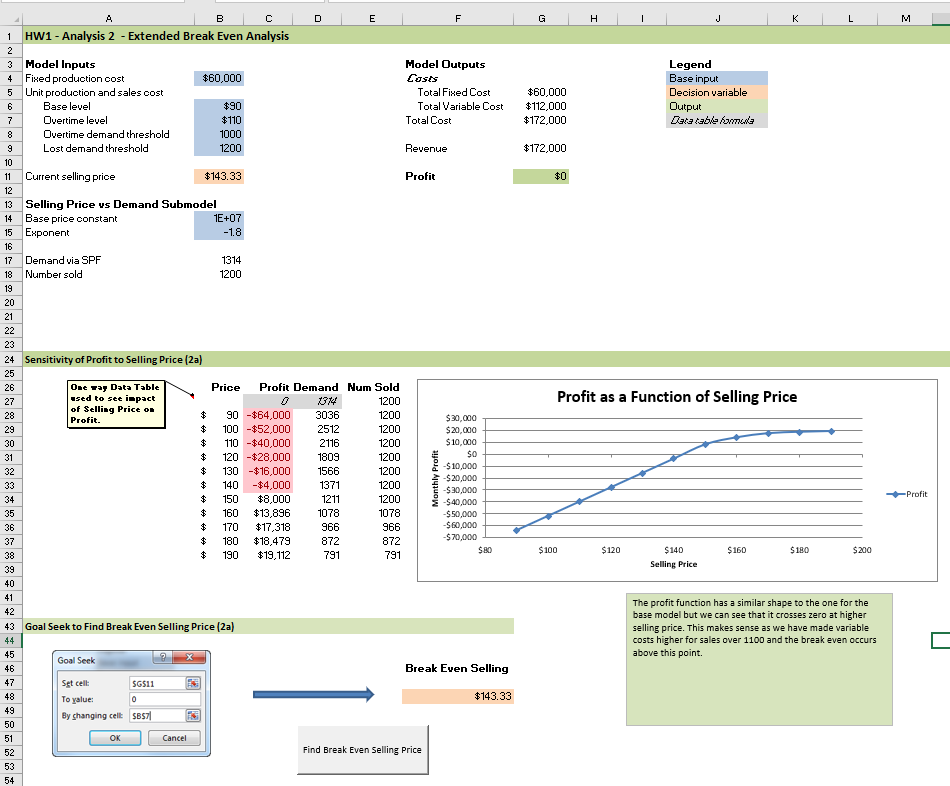
\includegraphics[width=1.0\textwidth]{images/output_2_0.png}
	\end{minipage}
	\caption{Typical spreadsheet model}
	\label{fig:xl_model}
\end{figure}

We then introduce a similar modeling problem that will be the focus of the rest of the notebook. The Walton Bookstore problem appears in the chapter on Monte-Carlo simulation in textbooks that I have used in my spreadsheet modeling course \cite{albrightBusinessAnalyticsData2016,winstonPracticalManagementScience2018}. The (slightly modified) problem is as follows:

\begin{itemize}
	\item we have to place an order for a perishable product (e.g. a calendar),
	\item there is a known unit cost for each unit ordered,
	\item we have a known and fixed selling price,
	\item demand is uncertain but we can model it with some simple probability distribution,
	\item for each unsold item, we can get a partial refund of our unit cost,
	\item we need to select the order quantity for our one order for the year; orders can only be in multiples of 25.
\end{itemize}

The overall goal is to build a Python based version of this model that will allow us to do sensitivity analysis, find the break even point for demand and analyze the problem using Monte-Carlo simulation.

\subsubsection{Build first model - procedural approach}
 
We start with a very simple model that ignores the uncertainty in demand and that is not object oriented. Proceeding much like we would in Excel, base input values are stored in variables. 

\begin{tcolorbox}
\begin{minted}[gobble=0]{python}
# Base inputs
unit_cost = 7.50
selling_price = 10.00
unit_refund = 2.50

# Demand parameters
demand_mean = 193
demand_sd = 40

# Deterministic model
demand = demand_mean

# Initial value for order quantity - this is the decision variable
order_quantity = 200
\end{minted}
\end{tcolorbox}

Students are given skeleton code as scaffolding and must finish the expressions for computing key intermediate outputs (\code{order\_cost, sales\_revenue, refund\_revenue}) and the final output, \code{profit}. Answers are provided at the bottom of the notebook so that students can attempt to finish the code but have a resource to correctly complete the code and move on. The screencast associated with the notebook also shows me completing the code in a subsequent code cell. Using skeleton code in this way has worked well both for lab based versions of this type of course as well as for online asynchronous versions.

\begin{tcolorbox}
\begin{minted}[gobble=0]{python}
order_cost = unit_cost * order_quantity
sales_revenue = ??? * selling_price
refund_revenue = ??? * unit_refund
profit = sales_revenue + refund_revenue - order_cost
\end{minted}
\end{tcolorbox}

At this point we discuss a fundamental difference between the computing model of Excel and that of Jupyter notebooks -- while spreadsheets respond automatically to changes, Jupyter notebooks require rerunning all code cells that include or follow the changed code. This difference in behavior between Jupyter notebooks and spreadsheets might be one of the most important concepts for students to internalize. A well known challenge associated with computational notebooks is the ease of running code cells out of order and introducing inadvertent errors. This point along with strategies to avoid it are discussed during the first week of the course which focuses on \href{http://www.sba.oakland.edu/faculty/isken/courses/mis6900/jupyter_notebooks.html}{notebook computing best practices as well as a historical look} at computational notebooks.
\subsubsection{Sensitivity analysis}

Since order quantity is the key decision variable, we might want to see how profit changes for different order quantities. In Excel, the Data Table tool provides an easy way to do this and is a staple of spreadsheet based management science textbooks. In a Data Table, a range of order quantities can be used as row or column input and one or more output values can be computed. In Python, the vectorized nature of the \href{https://numpy.org/}{NumPy} library \cite{NumPy}provides a simple way to accomplish the same thing. A range of order quantities is created as a NumPy array that can be used directly to compute vectors of all of the intermediate and final output variables. Much like Data Tables, vectorized computations avoid having to explicitly iterate, or loop, through a collection of input values.

A natural next step is to do the equivalent of an Excel 2-way Data Table. By creating a profit function that takes all of the base inputs as arguments, a list comprehension can then be used to generate the equivalent of a 2-way Data Table. Even better, this actually allows us to do the equivalent of an n-way Data Table with an arbitrary number of outputs -- something Excel does not have. This example provides an effective way to show the power of creating reusable functions and Python's handy list comprehension construct.

This code chunk,

\begin{tcolorbox}[left=0mm]
\begin{minted}[gobble=1]{python}
	def bookstore_profit(unit_cost, selling_price, 
	                     unit_refund, order_quantity, demand):
	'''
	Compute profit in bookstore model
	'''
		order_cost = unit_cost * order_quantity
		sales_revenue = np.minimum(order_quantity, demand) * selling_price
		refund_revenue = np.maximum(0, order_quantity - demand)
		profit = sales_revenue + refund_revenue - order_cost
		return profit
	
	# Set up input vector ranges	
	demand_range = np.arange(50, 301, 5)
	order_quantity_range = np.arange(50, 301, 25)
	
	# Create data table (as a list of tuples)
	data_table_1 = [(d, oq, bookstore_profit(
	                 unit_cost, selling_price, unit_refund, oq, d)) 
	for d in demand_range for oq in order_quantity_range]
	
	# Convert to dataframe
	dtbl_1_df = pd.DataFrame(data_table_1, 
	                         columns=['Demand', 'OrderQuantity', 'Profit'])
	
\end{minted}
\end{tcolorbox}

results in the following output:

% TODO - add output listing and plot

\begin{tcolorbox}
	\begin{verbatim}
	   Demand  OrderQuantity  Profit
	      50             50   125.0
	      50             75   -37.5
	      50            100  -200.0
	      50            125  -362.5
	      50            150  -525.0
	      ...
	     300            275   687.5
	     300            300   750.0
\end{verbatim}	
\end{tcolorbox}

\subsubsection{The object nature of Python}

It is not clear whether this non-object oriented approach will end up making the most sense for doing spreadsheet type modeling in Python. This uncertainty is made explicit in the notebook and students are led on a bit of a journey of discovery as we explore different software designs for this modeling problem. I purposefully designed the notebooks in this way to show students that the path to a solution is not necessarily linear and that giving yourself the freedom to explore alternatives, many of which will be dead ends, can lead to a rich learning experience. It is also more realistic in the sense that this is how most real problems are solved. It is analogous to the idea that mathematical proofs usually do not reflect the myriad of failed approaches that were tried but that ultimately contributed to the final product.

In preparation for building an object oriented version of the model, basic object concepts are reviewed. Since most students have done some Excel VBA programming in a previous course, I refer back to a few properties and methods of the Excel \code{Worksheet} object. In Python, everything is an object. Using Python lists as an example, we explore some of its attributes such as methods for appending items to a list and reversing the order of its elements. The \code{dir} function is used to see all of an object's attributes and we see that even things like integers are objects in Python. With this basic object refresher, we are ready to do some actual object oriented programming and create our own classes.

\subsubsection{Creating an object oriented model}

For our initial design of a \code{BookstoreModel} class we make all of the base inputs class attributes (properties) and then add method attributes to compute outputs such as costs, revenues and profits. Students can easily see the mapping between elements in the initial procedural model and this new object oriented version. Several important concepts and syntactical details of doing object oriented programming Python are highlighted. Again, the goal is to weave in these more advanced Python programming concepts within the context of a very familiar modeling problem. This section of the notebook ends with using the \code{BookstoreModel} class to create a new model object instance with all of its base inputs instantiated with values. Before moving, on students are presented with a few challenges involving enhancements to the \code{BookstoreModel} class. Interspersing short coding challenges throughout the notebook gives students a chance to test themselves on their understanding and to get some coding practice.

A few design dilemmas are posed and some non-working approaches illustrated as we try to decide on how to implement an n-way data table function for this new object oriented model. These meta reflections are intentionally included to better mimic actual software development and reinforce the idea that software development is much more than simply writing code to implement a perfectly thought out design. We forge ahead with some preliminary ideas and are confronted with an intermediate problem related to generating a list of dictionaries that represent combinations of inputs, or \textit{scenarios}, to evaluate. This provides a great opportunity to remind students of one of the great strengths of the open source software ecosystem -- we can leverage work done in other packages and even look at actual source code to see how something was implemented. In this case, the well known \href{https://scikit-learn.org/stable/}{scikit-learn} package \cite{ScikitlearnMachineLearning} has a \code{ParameterGrid} function that solves our scenario generation problem quite nicely. This example also reminds the students of the value of being able to make sense of API documentation and of object oriented code written by others. 

This first notebook draws to a close with the creation of a \code{data\_table} function that allows us to do sensitivity analysis with the objected oriented model. The payoff is the creation of the following faceted plot showing how profit varies for different order quantities and demand levels. We recap the main things learned in this notebook and prepare to add goal seeking capability to our model.

\begin{figure}[!ht]
	\centering
	\begin{minipage}{.80\textwidth}
		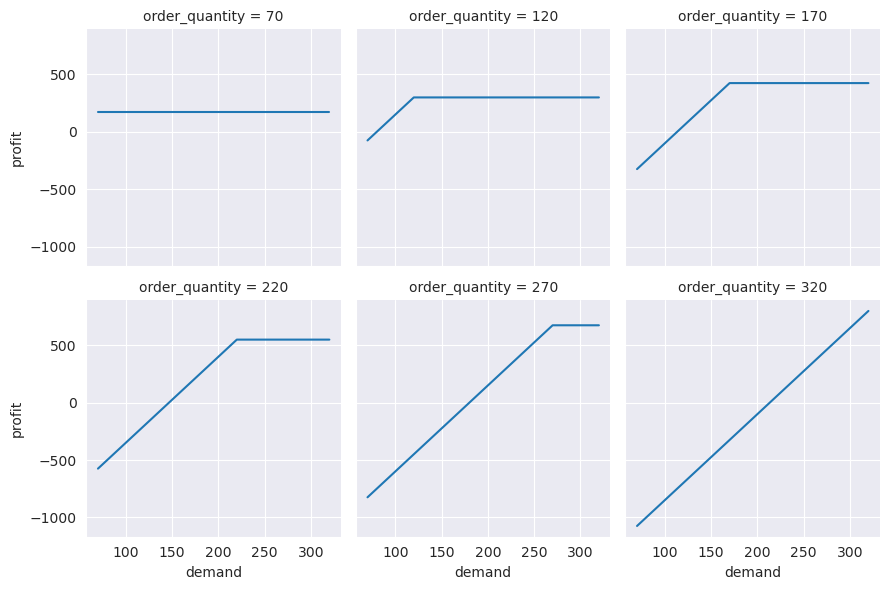
\includegraphics[width=1.0\textwidth]{images/two_way_dt.png}
	\end{minipage}
	\caption{Plot based on 2-way data table}
	\label{fig:2way_dt}
\end{figure}


\subsection{Notebook 2: Goal seek}

No self respecting modeling tool would be complete without goal seeking capability to do things such as finding the break even demand point in the bookstore model. For many students, Excel's Goal Seek tool can seem almost magical when encountered for the first time. Even after they get a sense of what it is doing, understanding the importance of the initial solution guess and how it can lead to Goal Seek reporting different solutions, is not very transparent. With Python, students can gain a much better understanding of how tools like Goal Seek really work. 

Before trying to build our \code{goal\_seek} function we take a brief detour into basic root finding algorithms through packages like \href{https://docs.scipy.org/doc/scipy/tutorial/optimize.html#root-finding}{SciPy} \cite{SciPy} as well as in \href{https://github.com/patrickwalls/mathematical-python/}{open source notebooks and scripts} that are widely available in the Python data science ecosystem \cite{wallsMathematicalPython2023}. We compare the output of Excel's Goal Seek with different starting values to the values obtained by different root finding algorithms implemented in Python. The importance of starting values and also the range of different root finding algorithms available is often surprising to business students who have spent most of their analytical life in Excel.

A \code{goal\_seek} function is created that implements a simple bisection search and we use it to find the break even demand point in our bookstore model. With \code{data\_table} and \code{goal\_seek} functions implemented, we are ready to move on to doing Monte-Carlo simulation.

\subsection{Notebook 3: Monte-Carlo simulation}

In the Excel modeling world, Monte-Carlo simulation can be done without add-ins, but packages like @Risk \cite{RISKRiskAnalysis} can make the process much easier. In particular, random variable generation for a wide range of probability distributions is facilitated by add-ins like @Risk. In Python, the NumPy package provide random variate generation for a large number of distributions and similarly, SciPy provides functions for computing distribution related quantities for many probability distributions. Much like we did when creating the \code{data\_table} function, we start with adding uncertainty to a single input variable in the bookstore model and rely on NumPy's vectorized computing capabilities to generate the profit associated with each realization of the random input. Then we can do standard statistical analysis of the simulation output using Python packages such as pandas and SciPy. In spreadsheet based simulation textbooks, the notion of the ``Flaw of Averages'' popularized by Sam Savage \cite{savageFlawAveragesWhy2012} is often illustrated. We do the same with our Python based model, showing how replacing random demand by its mean can result in a wildly optimistic estimate of the mean profit found through analyzing the simulation output. Much like doing simulation in Excel without add-ins, using Python makes transparent the quite simple and brute force nature of Monte-Carlo simulation.

Moving on to multiple uncertain inputs raises challenges much like those we faced when moving from a 1-way to an n-way data table function. In addition to modeling multiple uncertain inputs, we want to be able to specify a range of scenarios to run, much like we did for the \code{data\_table} function. The following set of design criteria are presented for a \code{simulate} function.

\begin{itemize}
	\item
	The first argument will be a model object (i.e.~something like the
	\code{BookstoreModel} model) that contains an \code{update}
	method. Soon, we should add an abstract \code{Model} class from
	which specific models such as the \texttt{BookstoreModel} class can be
	created. The abstract class will contain the \code{update} method.
	\item
	The random inputs will be passed in as a dictionary whose keys are the
	input variables being modeled as random and whose values are an
	iterable representing the draws from some probability distribution.
	Structurally, this is similar to how inputs are specified in the
	\code{data\_table} function.
	\item
	We can optionally pass in a dictionary of scenario inputs. This is
	exactly like the \code{data\_table} variable input.
	
	\begin{itemize}
		\item
		If no scenario input dictionary is passed in, a single simulation
		scenario is run using the current input values in the model object,
		\item
		If a scenario input dictionary is passed in, then a simulation
		scenario is run for every combination of parameters in the
		dictionary. Again, this is just like we do in the
		\code{data\_table} function.
	\end{itemize}
	\item
	The output will be a set of dictionaries containing dataframes of
	simulation output as well standard summary stats and plots.
\end{itemize}

This is followed by a well commented first attempt at a \code{simulate} function. By this point, students are well equipped to understand the code as it builds on basic Python concepts and more advanced concepts that we have already covered in the EwP module. The rest of the notebook is spent trying out the \code{simulate} function and ends with creating a grouped boxplot that many of them have likely created before with @Risk along with a faceted plot of histograms of profit created with the popular \href{https://seaborn.pydata.org/}{Seaborn} package.

\begin{figure}[!ht]
	\centering
	\begin{minipage}{.80\textwidth}
		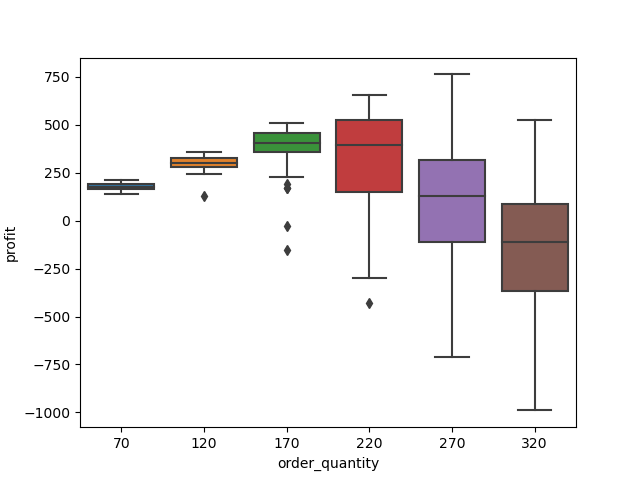
\includegraphics[width=1.0\textwidth]{images/boxplots.png}
	\end{minipage}
	\caption{Profit boxplots by order quantity}
	\label{fig:2way_dt}
\end{figure}

The first submodule and its three notebooks are very much about the type of modeling typically done in a spreadsheet based course. In a spreadsheet based course, students learn numerous Excel functions and techniques in the process of building and exercising such models. Similarly, numerous Python techniques are scattered throughout the three modeling focused notebooks. Now we shift gears and move beyond what might be considered prototyping and into the realm of deployment. The notebook ends with these thoughts.

\begin{tcolorbox}
	\begin{quotation}
		
\textsf{We have added a basic \code{simulate} function to our \code{data\_table} and \code{goal\_seek} functions. Python is proving to be quite nice for doing Excel-style "what if?" analysis.} 

\textsf{In Part 4 of this series, we'll make some improvements and do some clean-up on our classes and functions. We'll move everything into a single \code{whatif.py} module and learn how to create a Python package to make it easy to use and share our new functions. We'll try out our package on a new model and sketch out some ideas for future enhancements to the package. It's important we also start creating some basic documentation and a user guide.}
\end{quotation}
\end{tcolorbox}

\section{Submodule 2: The packaging and documentation notebooks}

%TODO - Need transition opening from modeling to packaging for reusability

Don't want to be copying and pasting code for the next model. We have spent some effort in creating something that is reusable.
VBA for Modelers got into the deployment process in the Excel world.

Classroom based spreadsheet modeling problems often end here. The model is built and used to analyze a given problem.

Creating a deployable Python package is a good exercise in designing and creating a reusable software artifact. Thinking about how others will interact with your software usually leads to better designed software.  In this submodule we create a Python package that can be imported and used by other modelers. This will require some design changes to our software and will also involve moving code out of Jupyter notebooks and into Python script files. While Jupyter notebooks can be integrated into production environments \cite{netflix}, it is much more common for code to live in Python script files. In addition to creating a deployable package, this submodule also discusses the importance of documentation in its many forms in a Python project.

% REMOVED
% Basic software engineering practices are often overlooked in business analytics classes but are certainly desirable in the professional world.

\subsection{Notebook 4: Project packaging}

The first notebook in this submodule starts by explaining what Python packages are and their role in sharing code. We then revisit a concept from earlier in the course -- creating a good project folder structure. For this we use what is known as a \href{https://cookiecutter.readthedocs.io/en/stable/}{cookiecutter} that can automatically generate a project folder structure and key files from the answers to a few prompts \cite{CookiecutterBetterProject}. There are a few different folder layouts used in Python projects and there is a bit of discussion on the folder structure we will use and resources given for exploring this issue further. Students are reminded of the importance of version control and we initialize a git repository for our budding package. The basics of version control were already covered in the first week of the course. My experience is that most students have little exposure to software project management concepts such as project folder structures and version control. This can lead to a jumble of files with incoherent names used as a proxy for version control -- \code{whatif\_v1.py}, \code{whatif\_v2.py}, \code{whatif\_final.py}, \code{whatif\_finalfinal.py}, and so on.

Key software design changes are then made which will make our code easier on our users. These changes include creating an abstract \code{Model} base class from which different model classes can be created and moving the \code{data\_table}, \code{goal\_seek}, and \code{simulate} functions into the \code{Model} base class as methods. All of the code is moved into a code module named \code{whatif.py}. Students are now ready to learn about the basics of turning our code into an installable package. This requires a basic understanding of two key Python files that are ubiquitous in Python pacakges - \code{\_\_init\_\_.py} and \code{setup.py}. Options are presented for installing our package locally so that we can use it for different modeling projects. This includes an explanation of how and where Python searches for packages when \code{import} statements are encountered in code. We defer discussion of uploading our package to a public code sharing platform such as PyPI. All of this can be quite complex and I have made every effort to distill things down to a minimal level of complexity needed to convey the important points. I stress that there is much complexity lurking here and it is something they will need to revisit time and time again.

This notebook ends by pointing the students to another notebook in which our newly deployed whatif package is used for a completely different model -- the New Car Simulation that has been a staple of Winston and Albright's textbooks for many years \cite{winstonPracticalManagementScience2018,albrightBusinessAnalyticsData2016}. This new model differs structurally from the Bookstore Model, but is representative of many financial models in that cash flows over multiple years need to be computed and summarized. 

\subsection{Notebook 5: Documentation}

This deployment focused submodule ends with a short notebook discussing the different types of documentation needed in a typical project. This includes code comments, docstrings, \code{readme} files and generating documentation by writing \href{https://www.sphinx-doc.org/en/master/usage/restructuredtext/basics.html}{reStructuredText} files (similar but more powerful than markdown) and using \href{https://www.sphinx-doc.org/en/master/index.html}{Sphinx}, the Python documentation generation tool. This is one of those tasks that few people like to do but can be very important for the long term success of a project. Even if you are just creating a tool for yourself, you will forget the details over time and documentation can be very beneficial in refreshing your memory. 

\section{Submodule 3: Excel data wrangling with Python}

The EwP module ends with what has become a relatively common use of Python with Excel -- automating various Excel data wrangling tasks. Examples include:

\begin{itemize}
	\item
	You have a whole folder full of csv (or Excel) files with the same
	file structure and you need to combine them into a single file. You
	might also need to make some changes to the consolidated file.
	\item
	You have an Excel file with multiple sheets of similarly structured
	data and you want to consolidate them into a single sheet.
	\item
	You have an Excel file with data in ``wide'' format and you need to
	convert it to long format, and then perhaps export out individual
	files (one per the key column(s) in the long formatted data).
	\item
	You have an Excel file acting as a simple flatfile database.
	Periodically, you get new Excel files that need to get appended to the
	``database'' file.
\end{itemize}

A single Jupyter notebook is used to give a taste of using Python to automate the process of working with Excel files by tackling each of the four examples above. Each of these examples are based on a real problems I encountered either in research or industrial projects. Several web based resources are shared including the \href{https://pbpython.com/}{Practical Business Python blog} written by Chris Moffitt, a data analytics professional \cite{moffittPracticalBusinessPython}. This blog, which focuses on helping Excel centric analytics professionals transition some of their work to Python, includes numerous posts on different aspects of Python and Excel integration.  

There are a number of Python based tools that either include functionality for working with Excel files or are dedicated to specific Excel related operations. These include:

\begin{itemize}
	\item
	pandas -
	\href{https://pandas.pydata.org/docs/reference/api/pandas.read_excel.html}{read\_excel},
	\href{https://pandas.pydata.org/docs/reference/api/pandas.ExcelWriter.html}{ExcelWriter},
	\href{https://pandas.pydata.org/docs/reference/api/pandas.DataFrame.to_excel.html}{to\_excel}
	\item
	\href{https://openpyxl.readthedocs.io/en/stable/}{openpyxl} - can
	read, write, and modify Excel files
	\item
	\href{https://xlsxwriter.readthedocs.io/}{XlsxWriter} - powerful but
	cannot edit existing Excel files
	\item
	\href{https://www.xlwings.org/}{xlwings} - provides ``glue'' between
	Python and Excel
\end{itemize}


\subsection{Example 1: Concatenating many csv files}

While this first example is not necessarily Excel related, using Excel to consolidate csv files through a series of manual Copy-Paste operations is something that many Excel users will admit to having done. After getting familiar with pathlib, a library for working with file systems which has recently been added to Python's standard library, students are led through the development of a short procedure that creates a list of the csv files to concatenate and then uses pandas to read and combine the files in a \code{DataFrame} and writes out the consolidated data as a csv file.

\subsection{Example 2: Consolidating data from multiple sheets in a Excel file using pandas}

Two different approaches are shown to consolidate data from multiple sheets into a single sheet. One approach uses pandas while the other relies on a library specifically created for working with Excel files from Python, openpyxl \cite{bibid}. One advantage to using Python rather than Visual Basic for Applications for this task is that Python is well suited for working with data in many different formats including csv, json, xml and a myriad of database formats. The Excel file may be just one data source out of a collection of data sources that are used to create some sort of combined database. The generality of Python is a strength in such scenarios.

\subsection{Example 3: Dealing with wide data and a multi-row header}

Reshaping data \cite{bibid} from wide to long is a common data wrangling task especially in preparation for plotting. In this example, not only do students have to grapple with reshaping the data in an Excel workbook, they also have to deal with the all too common problem of multi-row header lines in a spreadsheet. Excel's flexibility makes it easy to create such multi-row headers and pity the poor analyst who then has to deal with it when trying to move the data into some sort of data frame or database table. This example is posed as a challenge to the students. Examples of the desired outputs are shown and a few hints given. The answer is provided at the end of the notebook. This example really shows the power of Python in creating a reproducible and automated approach to dealing with a poorly structured Excel workbook, creating not only restructured data frames but also non-trivial plots. Attempting to do all of this in Excel, even with VBA, is not an easy task.

\subsection{Example 4: Appending new spreadsheet data in a consolidated Excel workbook}

Excel is not a database. Of course, that does not stop people from using it as a simple flat-file database. In such a scenario, it is not uncommon to have to periodically append new data to the end of a range of data in an Excel workbook. Again, a combination of openpyxl and pandas allows us to meet this challenge.

\subsection{More on Python/Excel integration}

The examples above barely scratch the surface of the use cases for Python integration with Excel. Our notebook ends with a shout out to the highly regarding Practical Business with Python blog and a list of specific examples that students can explore on their own.

\begin{itemize}
	\item
	\href{https://pbpython.com/excel-file-combine.html}{Combining Data
		From Multiple Excel Files} - file globbing, concatenating dataframes,
	\item
	\href{https://pbpython.com/pandas-excel-range.html}{Reading Poorly
		Structured Excel Files with Pandas} - advanced use of
	\texttt{read\_excel}, accessing ranges and Tables
	\item
	\href{https://pbpython.com/excel-pandas-comp.html}{Common Excel Tasks
		Demonstrated in Pandas} - totals rows, fuzzy string matching
	\item
	\href{https://pbpython.com/excel-pandas-comp-2.html}{Common Excel
		Tasks Demonstrated in Pandas - Part 2} - selection and filtering
	\item
	\href{https://pbpython.com/improve-pandas-excel-output.html}{Improving
		pandas Excel output} - using XlsxWriter to format Excel workbooks from
	Python
	\item
	\href{https://pbpython.com/advanced-excel-workbooks.html}{Creating
		Advanced Excel Workbooks} - XlsxWriter, inserting VBA from Python(!),
	using COM to merge sheets
	\item
	\href{https://pbpython.com/xlwings-pandas-excel.html}{Interactive Data
		Analysis with Python and Excel} - using xlwings to ``glue'' Python and
	Excel together, using sqlalchemy to interact with databases
\end{itemize}

% todo Check the hyperlinks above

\section{Classroom experience and the future}

This module has been included in my Advanced Analytics with Python course for the past three years. The course is offered in a seven-week accelerated format during May and June. It is an online and asynchronous course. The EwP module is covered over the course of two weeks and is the subject of one of the major homework assignments for the semester. The first part of the assignment involves creating a basic model, similar in complexity to the Bookstore Model, and doing sensitivity analysis, goal seeking and simulation with the model. It requires the students to import and use the \code{whatif.py} package we created as part of the module. The second part of the assignment is based on the last submodule and requires  students to complete a task involving creation of a multi-sheet Excel workbook from a set of csv files using Python. Then, using the openpyxl library, they have to create and add formulas to the workbook and format them properly. The ranges used in the formulas vary by sheet and require determination of the number of rows in each sheet of data and use that information to construct the appropriate formula. An example assignment is available from \href{some.url}{here}. The module has been well received and several of the working students have reported back to me that they have found use cases for these techniques in their day to day analytical activities.

Rumors have swirled for a number of years that Microsoft was considering adding Python as a first class language alternative to VBA within their MS Office suite of packages \cite{bibid}. While this has not yet materialized, there continues to be significant interest in using Python to manipulate not only Excel workbooks but other office documents such as Powerpoint presentations \cite{bibid}. Given that business students are very familiar with both Excel and Powerpoint, inclusion of this material in a business school Python based analytics course seems quite appropriate. Students can learn more advanced and extremely useful Python concepts and techniques within a context with which they are intimately familiar. Manipulation of MS Office directly relevant to the job content of many of the students. This teaching module is a natural follow up to the commonly taught spreadsheet based analytics courses found in many business schools and provides an interesting way to teach and learn Python for analytics.

\section{Random notes}
Learning good Python programming practices via learning to model in similar way that students learn good spreadsheet practices through building spreadsheet models using the W\&A textbook.

%https://www.bleepingcomputer.com/news/microsoft/microsoft-considers-adding-python-as-an-official-scripting-language-to-excel/

%https://www.reddit.com/r/excel/comments/lrw21h/will_ms_excel_ever_use_python_as_scripting/




% Acknowledgments here
\ACKNOWLEDGMENT{%
% Enter the text of acknowledgments here
}% Leave this (end of acknowledgment)


% Appendix here
% Options are (1) APPENDIX (with or without general title) or 
%             (2) APPENDICES (if it has more than one unrelated sections)
% Outcomment the appropriate case if necessary
%
% \begin{APPENDIX}{<Title of the Appendix>}
% \end{APPENDIX}
%
%   or 
%
% \begin{APPENDICES}
% \section{<Title of Section A>}
% \section{<Title of Section B>}
% etc
% \end{APPENDICES}


% References here (outcomment the appropriate case) 

% CASE 1: BiBTeX used to constantly update the references 
%   (while the paper is being written).
\bibliographystyle{informs2014} % outcomment this and next line in Case 1
\bibliography{python_excel.bib} % if more than one, comma separated

% CASE 2: BiBTeX used to generate mypaper.bbl (to be further fine tuned)
%\input{mypaper.bbl} % outcomment this line in Case 2

\end{document}


